\chapter{Изучение предметной области}

\section{Технология блокчейн}

Блокчейн (blockchain) — база данных, состоящая из последовательно выстроенной цепочки цифровых блоков, в каждом из которых хранится собственная хеш-сумма и хеш-сумма предыдущего блока.

Данная концепция была предложена в анонимно опубликованной статье «Bitcoin: A Peer-to-Peer Electronic Cash System», изложив основы для создания децентрализованной и прозрачной электронной валюты, являющейся результатом обобщения нескольких направлений развития информационных технологий, таких как:

\begin{enumerate} 
  \item Технология одноранговой сети распределённого хранения и передачи файлов BitTorrent.
  
  \item Криптография открытого ключа, для обеспечения безопасности электронных коммуникаций.
  
  \item Технология хеширования, с помощью которой формируются заголовки каждого блока.
  
  \item Механизм «proof-of-work», разработанный Адамом Бэком для защиты от спама в электронной почте.
\end{enumerate}

Впервые данная технология была реализована в платежной системе в виде одноранговой сети — «Bitcoin», однако технология блокчейн может быть применена на любые взаимосвязанные информационные блоки, такие распределенные реестры пригодились не только для операций с криптовалютами, но и для создания децентрализованных баз данных, систем цифровой идентификации, бухгалтерского учета.

В данный момент блокчейн-технологии применяются в таких областях как, авторство и право владения, финансовые операции, сфера развлечений, интернет вещей, средства электронного голосования, и др.

Основные принципы блокчейна:

\begin{enumerate} 
  \item Распределенный реестр.
  
  \item Децентрализация и отказ о посредничества — в отношениях между двумя участниками нет третьих лиц.
  
  \item Децентрализация и отказ о посредничества — в отношениях между двумя участниками нет третьих лиц.
  
  \item Необратимость и устойчивость — невозможно удалить или изменить добавленные записи.
\end{enumerate}

Связь между блокчейном (on-chain) и внешним миром (off-chain) требует дополнительных элементов инфраструктуры, называемых оракулами.

Оракул в блокчейне — это элемент промежуточного программного обеспечения, который обеспечивает связь между различными блокчейнами и любой внешней средой.

\section{Механизмы консенсуса}

Еще до публикации статьи «Bitcoin: A Peer-to-Peer Electronic Cash System», многие пытались разработать цифровую наличность, используя цифровые подписи, как их неотъемлемую часть, сводя тем самым проблему создания цифровой наличности к проблеме двойной траты. Цифровая подписи не может гарантировать то, что она не будет использована повторно, таким образом, до 2008 года, состояние дел в этом области сводилось к тому, что все системы цифровых валют должны были быть централизованными.

Основные характеристики, которыми должны обладать механизм консенсуса:

\begin{enumerate} 
  \item Эквивалентность затрат — добыча блока должна создавать безвозвратные издержки, примерно эквивалентные вознаграждению за добычу блока.
  
  \item Самосертифицируемость — проверка должна осуществляться самостоятельно, внутри программного обеспечения, без привязки к чему-либо еще.
  
  \item Необратимость — затраты на добычу блока должны возникать в реальном мире, в результате процессов, которые не могут быть обратимы.
\end{enumerate}

\subsection{Механизм достижения консенсуса «proof-of-work»}

Идея механизма доказательство выполнения работы («proof-of-work») заключается в внедрении сжигания электричества, как доказательство того, что определенное количество электроэнергии было потреблено тем или иным узлом на выполнение работы. Доказательство выполнения работы ориентированно на нахождения решения по заранее известному алгоритму за некоторое конечное время.

Принцип работы механизма:

\begin{enumerate} 
    \item Все узлы могут генерировать лотерейные билеты.
    
    \item Сгенерированный лотерейные билеты криптографически связаны с их решением о том, какие транзакции они одобряют.
    
    \item «Стирание» лотерейного билета требует определенной вычислительной мощности.
    
    \item Из-за конструкции используемых алгоритмов, единственный способ раскрыть лотерейный билет — стереть его.
    
    \item Сеть определяет редкость принимаемых билетов.
    
    \item При предъявлении узлом билета с редкостью один на миллион, сеть делает вывод о том, что узел перебрал в среднем около миллиона лотерейных билетов.
    
    \item Сеть начисляет цифровую валюту узлам, предъявившим выигрышные лотерейные билеты.
    
    \item Поскольку лотерейные билеты привязаны к решениям об одобрении транзакций, узел, подтвердивший недорисованные транзакции, не сможет получить вознаграждение.
    
    \item Поскольку лотерейные билеты привязаны к решениям об одобрении транзакций, узел, подтвердивший недорисованные транзакции, не сможет получить вознаграждение.
    
    \item Для поддержания стабильности, сеть увеличивает редкость выигрышных билетов, если выигрыши происходят слишком часто, и понижает сложность, если предъявляемых выигрышных билетов становится мало.
\end{enumerate}

Преимущества механизма доказательство работы:

\begin{enumerate} 
  \item Низкое влияния доли цифровой валюты узла на возможность добычи.
  
  \item Держатели больших активов цифровой валюты на могут принимать решения за всю сеть.
  
  \item Высокая надежность, поскольку эффективная атака невыгодна на фоне высоких затрат.
\end{enumerate}

Недостатки механизма доказательства работы:

\begin{enumerate} 
  \item Для «стирания» лотерейного билета требуются большие вычислительные мощности, а постоянный рост сложности вычислений приводит к росту потребления электроэнергии, которая необходима мощным компьютерным системам. Использование углеводородного топлива для питания объединенной сети узлов приводит к росту экологической нагрузки.
  
  \item Потенциальная уязвимость перед атакой пятидесяти одного процента — может являться проблемой для маленьких блокчейнов с длительным временем обработки блоков.
\end{enumerate}

\subsection{Механизм достижения консенсуса «proof-of-stake»}

В механизме «proof-of-stake», предложенным как альтернатива затратному «proof-of-work», вместо подбора выигрышного числа, транзакции подтверждаются путем заморозки никоторого количества цифровой валюты в качестве обеспечения. Цифровая валюта заморожена до тех пор, пока не будет достигнута договоренность между большинством узлов о валидности транзакции. После достижения договоренности, путем голосования, транзакция добавляется в блокчейн, а цифровая валюта остается замороженной еще некоторое время, для защиты сети от двойной траты.

Принцип работы механизма:

\begin{enumerate} 
  \item Каждый узел может заблокировать цифровую валюту («staking»).
  
  \item Узлы могут проголосовать за действительный блок, подписав свой голос цифровой подписью.
  
  \item Побеждает тот блок, набравший наибольшее число голосов.
  
  \item Если поведение узлов окажется злонамеренным, они теряют всю заблокированную сумму.
\end{enumerate}

Ключевое преимущество механизма доказательство доли владения в том, что для проведения атаки требуются значительные средства, что делает ее нецелесообразной, поскольку атакующий сам пострадает от атаки, нарушив устойчивость валюты.

Главным недостатком механизма доказательство доли владения является то, что наказание за недобросовестное поведение является синтетическим и существует только внутри системы, из-за чего возникает проблема «ничего на кону». Атакующий может сделать создать более длинную альтернативную цепочку, посредством расходования «несуществующих» ресурсов, также его могут поддержать другие узлы, поскольку они не несут за это реальных трат, по итоге атакующий может осуществлять атаку «двойной траты», отклоняя определенные транзакции. Данная проблема является фатальной для успеха механизма «proof-of-stake».

\section{Сравнение централизованных, распределенных и децентрализованных приложений}

Программное приложение — это программное обеспечение, предназначенное для выполнение определенных задач и рассчитанное на непосредственное взаимодействие с пользователем.

Большинство существующих приложений реализуют централизованную модель взаимодействия клиент-сервер, некоторые из них используют распределенную модель доставки сообщений.

Централизованные системы непосредственно управляют данными во всей системе, а вся информация протекает через единый центр. Работа отдельных компонентов таких приложений зависит от возможности центра посылать и принимать информацию, а также осуществлять управление (рисунок \ref{fig:centralization}).

\begin{figure}[H]
\begin{center}
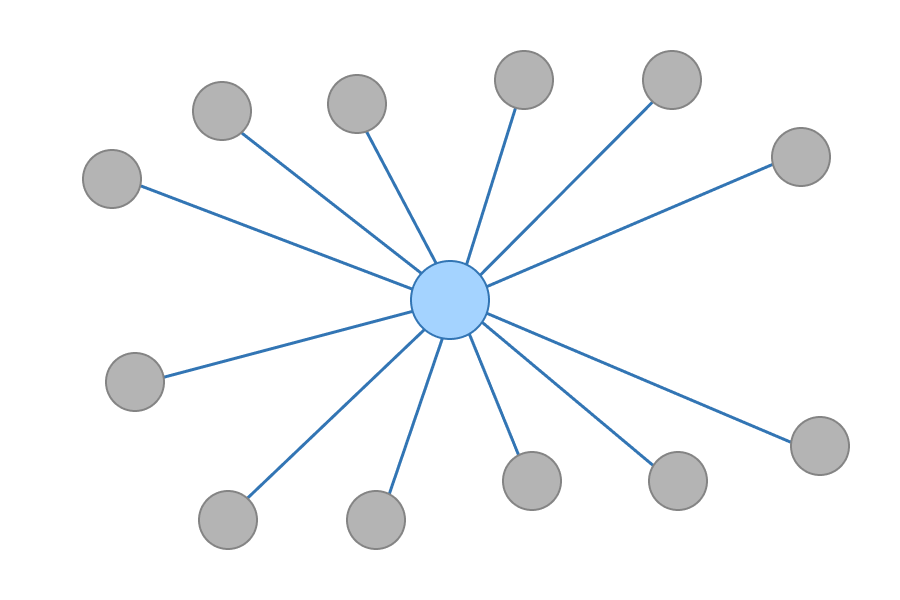
\includegraphics[width=0.7\hsize]{fig/centralization.png}\\[2mm]
\caption{Централизованная система}\label{fig:centralization}
\end{center}
\end{figure}

Децентрализованными называют системы, в которых отсутствуют узлы, управляющие другими узлами, иначе говоря, такая система полностью состоит из одноранговых узлов (рисунок \ref{fig:decentralization}).

\begin{figure}[H]
\begin{center}
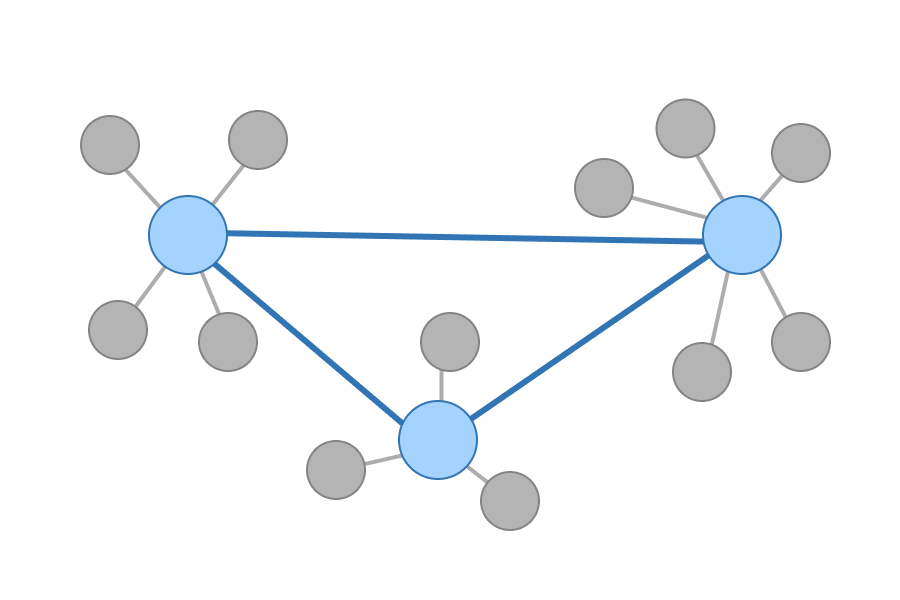
\includegraphics[width=0.7\hsize]{fig/decentralization.png}\\[2mm]
\caption{Децентрализованными система}\label{fig:decentralization}
\end{center}
\end{figure}

Распределенными называют системы, в которых вычислительная нагрузка и хранение данных распределяются между несколькими узлами (рисунок \ref{fig:cdn}).

\begin{figure}[H]
\begin{center}
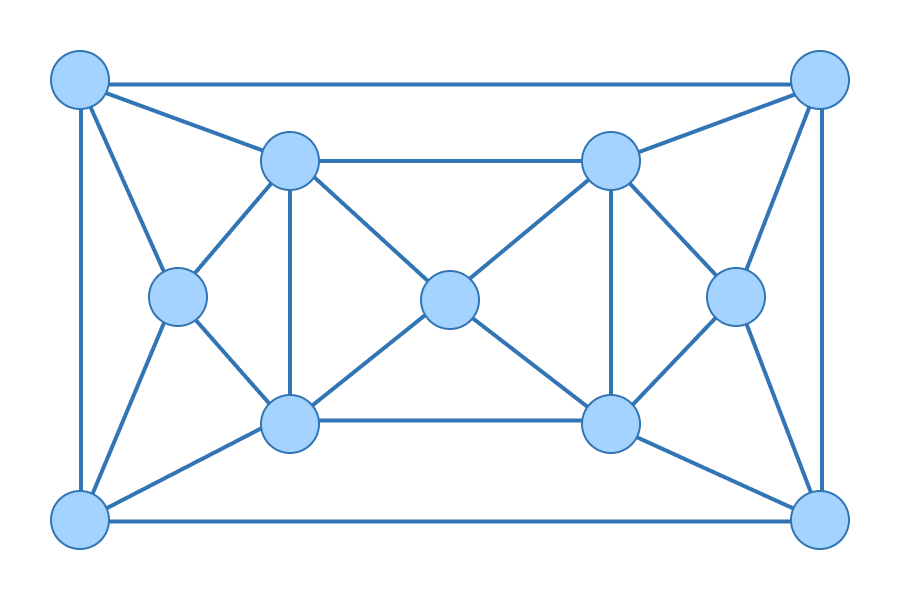
\includegraphics[width=0.7\hsize]{fig/cdn.png}\\[2mm]
\caption{Распределенная система}\label{fig:cdn}
\end{center}
\end{figure}

Таким образом, любая система, использующая цепочку блоков и пиринговые технологии, может быть одновременно распределенной и децентрализованной. Именно добавление технологии блокчейн к распределенной модели, сделало возможным создание «web3» приложений.

Особенности «web3» приложений:

\begin{enumerate} 
  \item Отсутствие центральной точки отказа — данные в децентрализованных приложения распределены между всеми узлами, при этом, узлы действуют независимо, если один из них остановится, другие продолжат работу в сети.
  
  \item Основной код и данные децентрализованных приложений хранится и выполняется в блокчейне.
  
  \item Как правильно, децентрализованный приложения имеют открытый исходный код.
\end{enumerate}

\section{Ethereum, как платформа для создания децентрализованных приложений}

Ethereum — распределенная, децентрализованная вычислительная инфраструктура c открытым исходным кодом которая выполняет программы, называемые смарт-контрактами.

Платформа Ethereum позволят разрабатывать децентрализованные приложения со встроенными экономическими функциями, обеспечивая высокую доступность и возможность аудита.

Компоненты платформы Ethereum:

\begin{enumerate} 
  \item Peer-to-peer сеть, работающая по протоколу DEVp2p.
  
  \item Правила консенсуса, определенные в справочной спецификации.
  
  \item Транзакции — сетевые сообщения, которые включают в себя отправителя, получателя, полезную нагрузку в виде данных и другую информацию.
  
  \item Виртуальная машина (Ethereum Virtual Machine) — обрабатывает переходы состояний в сети. Программы, написанные на языках высокого уровня, компилируются в байт-код для выполнения на EVM.
  
  \item Структура данных — состояние Ethereum хранится локально на каждом узле в виде базы данных.
  
  \item Алгоритм консенсуса — в данный момент Ethereum использует механизм консенсуса «PoW», однако в ближайшее время планируется совершить переход на «PoS».
\end{enumerate}

В Ethereum есть два типа учетных записей, внешние учетные записи (externally owned accounts) и контрактные учетные записи. EOT контролируются пользователями с помощью специальных клиентов, которые являются внешними по отношению к платформе Ethereum. Контрактные счета, напротив, контролируются программным кодом, который выполняется виртуальной машиной Ethereum, такие счета называют смарт-контрактами.

Смарт-контракты — неизменяемые компьютерные программы, которые детерминировано запускаются в контексте виртуальной машины Ethereum, как части сетевого протокола Ethereum.

Смарт-контракты пишутся на языках высокого уровня, например на Solidity, но для запуска они должны быть скомпилированы в низкоуровневый байт-код, который может выполняться EVM. После компиляции, смарт-контракт разворачивается на платформе Ethereum с помощью специальной транзакции, отправляемой на адрес \verb|0x0|.

Каждый контракт идентифицируется адресом Ethereum и может быть использован в транзакции в качестве получателя. Смарт-контракты выполняются только в случае, когда они вызываются транзакцией, физически, контракты бездействуют до тех пор, пока транзакция не инициирует выполнение какой-либо функции контракта.

Транзакции являются атомарными, они либо успешно завершаются, либо откатываются. Неудачные транзакции регистрируются в блокчейне, потраченный газ за попытку выполнить транзакцию списывается с учетной записи инициатора транзакции, однако, такие транзакции не оказывают никакого влияния на смарт-контракты.

В настоящее время, поддерживаемые языки для написания смарт-контрактов включают:

\begin{enumerate} 
  \item LLL — функциональный язык программирования с синтаксисом, подобным Lisp первый язык высокого уровня использованный для написания смарт-контрактов.
  
  \item Serpent — процедурным язык программирования с синтаксисом, подобным Python.
  
  \item Vyper — язык созданный чтобы приблизятся к чистому функциональному стилю программирования, подобным Python.
  
  \item Bamboo — язык разработанный под влиянием Erlang, с явными переходами состояния и без интеграционного управления, на данный момент не получит широкого распространения.
  
  \item Solidity — процедурный язык программирования с синтаксисом, подобным JavaScript и C++. Самый популярный язык для написания смарт-контрактов Ethereum.
\end{enumerate}

Solidity — объектно-ориентированный, предметно-ориентированный язык программирования созданный доктором Гэйвином Вудом в 2014 году, как язык, специально предношенный для написания смарт-контрактов с прямой поддержкой выполнения в децентрализованной среде, на данный момент разрабатывается и поддерживается как независимый проект с открытым исходным кодом.